\documentclass[12pt]{article}
\usepackage[utf8]{inputenc}
\usepackage{amsmath, amssymb}
\usepackage{geometry}
\usepackage{enumitem}
\usepackage{fancyhdr}
\usepackage{booktabs}
\usepackage{longtable}
\usepackage{array}
\usepackage{graphicx}
\usepackage{float}
\usepackage{hyperref}
\geometry{margin=1in}

\pagestyle{fancy}
\fancyhf{} % clear all header and footer fields
\renewcommand{\footrulewidth}{0.4pt} % adds a line at the top of the footer
\fancyfoot[R]{\thepage} % right-aligned page number

\setlength{\parindent}{0pt}
\setlength{\parskip}{0.5em}

% Reduce space before/after itemize/enumerate
\usepackage{enumitem}
\setlist{itemsep=0.1em, topsep=0.1em, leftmargin=2em}

\title{DBA5101: Estimation of Demand Function for Train Travel}
\author{}
\date{}

\begin{document}

\begin{titlepage}
    \centering
    \vspace*{1cm}
    {\Huge\bfseries DBA5101 Group Project\\[0.5em]}
    {\Huge Estimation of Demand Function for Train Travel \par}
    \vspace{1cm}
    
\includegraphics[width=0.30\textwidth]{nus_logo.png} \\[2em]
    {\large Group Members\par}
    \vspace{0.5cm}
    {\small
    CHAN HIU LOK \\[0.2em]
    CHEN HANGYU \\[0.2em]
    SANYA RAJPAL \\[0.2em]
    TANYA TOOLEY \\[0.2em]
    WANG YING \\[0.2em]
    }
    \vspace{1cm}
    {\large
    National University of Singapore \\
    \vspace{0.5cm}
    Submission Date: September 20, 2025 \\
    \vspace{0.3cm}
    \href{https://github.com/ying-jeanne/managerial_economics}{Link to code repository}
    }
    \vfill
\end{titlepage}
\thispagestyle{fancy}

% PAGE 1: INTRODUCTION & DATA OVERVIEW
\section{Introduction \& Data Overview}

This study estimates the demand function for train travel using 209,697 observations of ticket sales data. We address the fundamental endogeneity problem where price and quantity are simultaneously determined, causing standard OLS to underestimate true price sensitivity.

We apply both OLS and Two-Stage Least Squares (2SLS) using supply-side instruments (capacity constraints and route characteristics) for identification. OLS results suggest highly inelastic demand (elasticity $\approx$ -0.06 to -0.17), but 2SLS reveals substantially more price-sensitive demand (elasticity -0.96 to -1.61), confirming significant endogeneity bias.

\subsection{Data Overview}
Our dataset comprises 209,697 observations of train ticket sales with rich information on pricing, customer characteristics, and temporal patterns. Data quality is good with no significant missing values after date alignment and cleaning. 

Core variables include: num\_seats\_total, mean\_net\_ticket\_price, departure/purchase dates, train numbers, cumulative sales, cabin types, trip types, and customer categories.

\subsection{Descriptive Statistics}
Preliminary analysis reveals a negative correlation between price and quantity demanded (-0.19), consistent with economic theory. Customer segmentation shows distinct patterns: leisure travelers (Category B) more frequently choose normal cabins (isNormCabin = true) with correlation 0.45 and exhibit different booking timing compared to business travelers. They tend to book in advance, showing a +0.35 correlation with days\_to\_departure.

\begin{figure}[H]
    \centering
    
\includegraphics[width=1.0\textwidth,keepaspectratio]{basic_statistic.png}
    \caption{\small Key Variables Correlation Heatmap}
    \label{fig:basic_statistics}
\end{figure}

The correlation between price and trip types (correlation = 0.14) suggests that more expensive tickets are slightly more likely to be one-way trips.

Temporal analysis indicates strong seasonal patterns in both pricing and demand, with summer/winter months showing higher prices and different demand elasticity. The booking horizon variable exhibits non-linear effects, with demand patterns varying significantly between early bookings (60+ days), optimal booking windows (14--30 days), and last-minute purchases (\textless 7 days) as illustrated in (Appendix~\ref{app:season_choice}).

\section{Methodology \& Instrumental Variable Strategy}

\subsection{Demand Function Specification}
We estimate demand functions using both linear and log-linear specifications to capture different elasticity patterns:

\textbf{Linear Model:}
\begin{equation}
\text{quantity}_i = \beta_0 + \beta_1 \cdot \text{price}_i + \beta_2 \cdot \text{demand\_shifters}_i + \varepsilon_i
\end{equation}

\textbf{Log-Linear Model:}
\begin{equation}
\log(\text{quantity}_i) = \beta_0 + \beta_1 \cdot \log(\text{price}_i) + \beta_2 \cdot \text{demand\_shifters}_i + \varepsilon_i
\end{equation}

Demand shifters include log-transformed booking horizon (log\_days\_to\_departure), weekend departure indicators, customer segments (A or B), seasonal patterns, cabin type preferences, train type characteristics, trip type (one-way vs return), and interaction terms capturing customer-service combinations (Business×Premium, Individual×Premium, Business×Normal).

\subsection{Endogeneity Problem}
Standard OLS estimation faces a fundamental endogeneity challenge: price and quantity are simultaneously determined in equilibrium. High-demand periods lead to higher prices, creating positive correlation between unobserved demand shocks and price. This simultaneity bias typically causes OLS to underestimate the true price elasticity of demand.

The bias direction can be formalized as:
\begin{equation}
\text{plim}(\hat{\beta}_1^{OLS}) = \beta_1 + \frac{\text{Cov}(\text{price}, \varepsilon)}{\text{Var}(\text{price})}
\end{equation}

Since positive demand shocks increase both quantity and price, we have $\text{Cov}(\text{price}, \varepsilon) > 0$. Given that the true demand slope $\beta_1 < 0$, the positive bias term makes OLS estimates less negative than the true parameter: $\hat{\beta}_1^{OLS} > \beta_1$. This biases estimates toward zero, understating the magnitude of consumer price sensitivity.

\subsection{Feature Engineering \& Instrumental Variable Strategy}
Our identification strategy requires careful feature engineering to address endogeneity while capturing demand heterogeneity:

\textbf{Instrumental Variables (2SLS Only):}
Our identification strategy exploits supply-side variation that affects pricing but not passenger demand preferences:
\begin{itemize}
    \item \textit{Cumulative\_sales}: Nomally revenue management algorithms automatically adjust prices based on capacity utilization through predetermined rules, creating supply-side pricing variation independent of individual passenger preferences.
    \item \textit{Train\_Number\_All}: Route-specific operational characteristics (train type, service frequency, infrastructure) affect pricing through cost structures while being predetermined relative to individual demand decisions. (We need to convert it to dummies with one hot encoding)
\end{itemize}

\textbf{Control Variables (Both OLS \& 2SLS):}
\begin{itemize}
    \item Log booking horizon (\texttt{log\_days\_to\_departure}) captures diminishing booking effects better. The rationale is explained in (Appendix~\ref{app:days_log}).
    \item Seasonal patterns (\texttt{departure\_season}) control for systematic demand variations across seasons. It would be converted to dummies with one hot encoding. The choice of seasonal dummies over monthly dummies is justified in (Appendix~\ref{app:season_choice}).
    \item Customer segments, cabin types, weekend indicators, trip types, and train characteristics.
    \item Customer-service interactions (\texttt{Business\_x\_Premium}, \texttt{Individual\_x\_Premium}, \\
    \texttt{Business\_x\_NormCabin}).
\end{itemize}

\section{Results \& Analysis}

\subsection{Estimation Results Comparison}
We compare OLS (treating price as exogenous) with 2SLS (using supply-side instruments to correct endogeneity):

\begin{table}[H]
\centering
\caption{Demand Estimation Results: OLS vs 2SLS Comparison}
\begin{tabular}{lcccc}
\toprule
Method & Specification & Price Elasticity & R² & Bias Factor \\
\midrule
OLS & Linear & -0.0646 & 0.0897 & \- \\
OLS & Log-log & -0.1652 & 0.1406 & \- \\
2SLS & Linear & -1.6106 & -0.3558 & 24.9× \\
2SLS & Log-log & -0.9627 & -0.0341 & 5.8× \\
\bottomrule
\end{tabular}
\end{table}

\textbf{Specification Choice:} While both 2SLS specifications correct for endogeneity, we focus our economic interpretation on the log-log result (-0.96) rather than the linear specification (-1.61). This choice reflects methodological considerations detailed in Appendix~\ref{app:log_transform}, including superior distributional properties for the skewed quantity data, constant elasticity interpretation, and better accommodation of heteroskedasticity concerns inherent in our dataset.

\textbf{Endogeneity Bias Confirmation:} OLS systematically underestimates price sensitivity by factors as we discussed in section 2.2. The 2SLS with supply-side identification reveals substantially more elastic demand than naive OLS estimates suggest.

\subsection{Key Findings \& Validation}
\textbf{Endogeneity Correction:} 2SLS yields demand elasticity of -0.96 versus OLS estimate of -0.17, representing a 5.8× bias factor. This confirms substantial understatement of price sensitivity in standard estimation.

\textbf{Model Features:} Our specification accommodates demand heterogeneity through interaction terms and non-linear booking effects, though formal testing would strengthen validation of these patterns.

\textbf{Identification:} Supply-side instruments (capacity utilization, route characteristics) are theoretically sound, affecting pricing through cost structures while remaining predetermined relative to passenger demand.

\section{Economic Interpretation \& Conclusions}

\subsection{Economic Implications}
Our corrected elasticity estimates reveal train travel demand is significantly more price-sensitive than conventional wisdom suggests. Using our consistent log specification approach, 2SLS estimation yields a demand elasticity of approximately -0.96, indicating that consumers respond substantially to price changes: a 10\% price increase leads to approximately 9.6\% reduction in quantity demanded.

With an elasticity magnitude just below the unit elastic threshold ($|\varepsilon| = 0.96 < 1$), train travel exhibits moderately inelastic demand. This implies that while passengers are price-sensitive, price increases still generate net revenue gains for operators, though the revenue effect diminishes as elasticity approaches unity. The near-unit elasticity suggests significant competitive pressures in the rail transport market, with passengers having meaningful substitute options when prices rise.

\subsection{Conclusions}

From a methodological perspective, this analysis underscores the critical importance of addressing endogeneity in demand estimation and provides a robust framework for supply-side instrumental variable selection. The use of capacity constraints and route characteristics as instruments offers a promising approach for future transportation economics research.

\newpage
\appendix

\section{Log Transformation for Booking Horizon}\label{app:days_log}

We use log transformation for the booking horizon variable (\textit{log\_days\_to\_departure}) consistently across both OLS and 2SLS specifications for theoretical and practical reasons.

\textbf{Economic Rationale:} Dynamic pricing algorithms typically implement diminishing marginal adjustments as departure approaches, making log specification theoretically appropriate for capturing these non-linear pricing effects.

\begin{figure}[H]
    \centering
    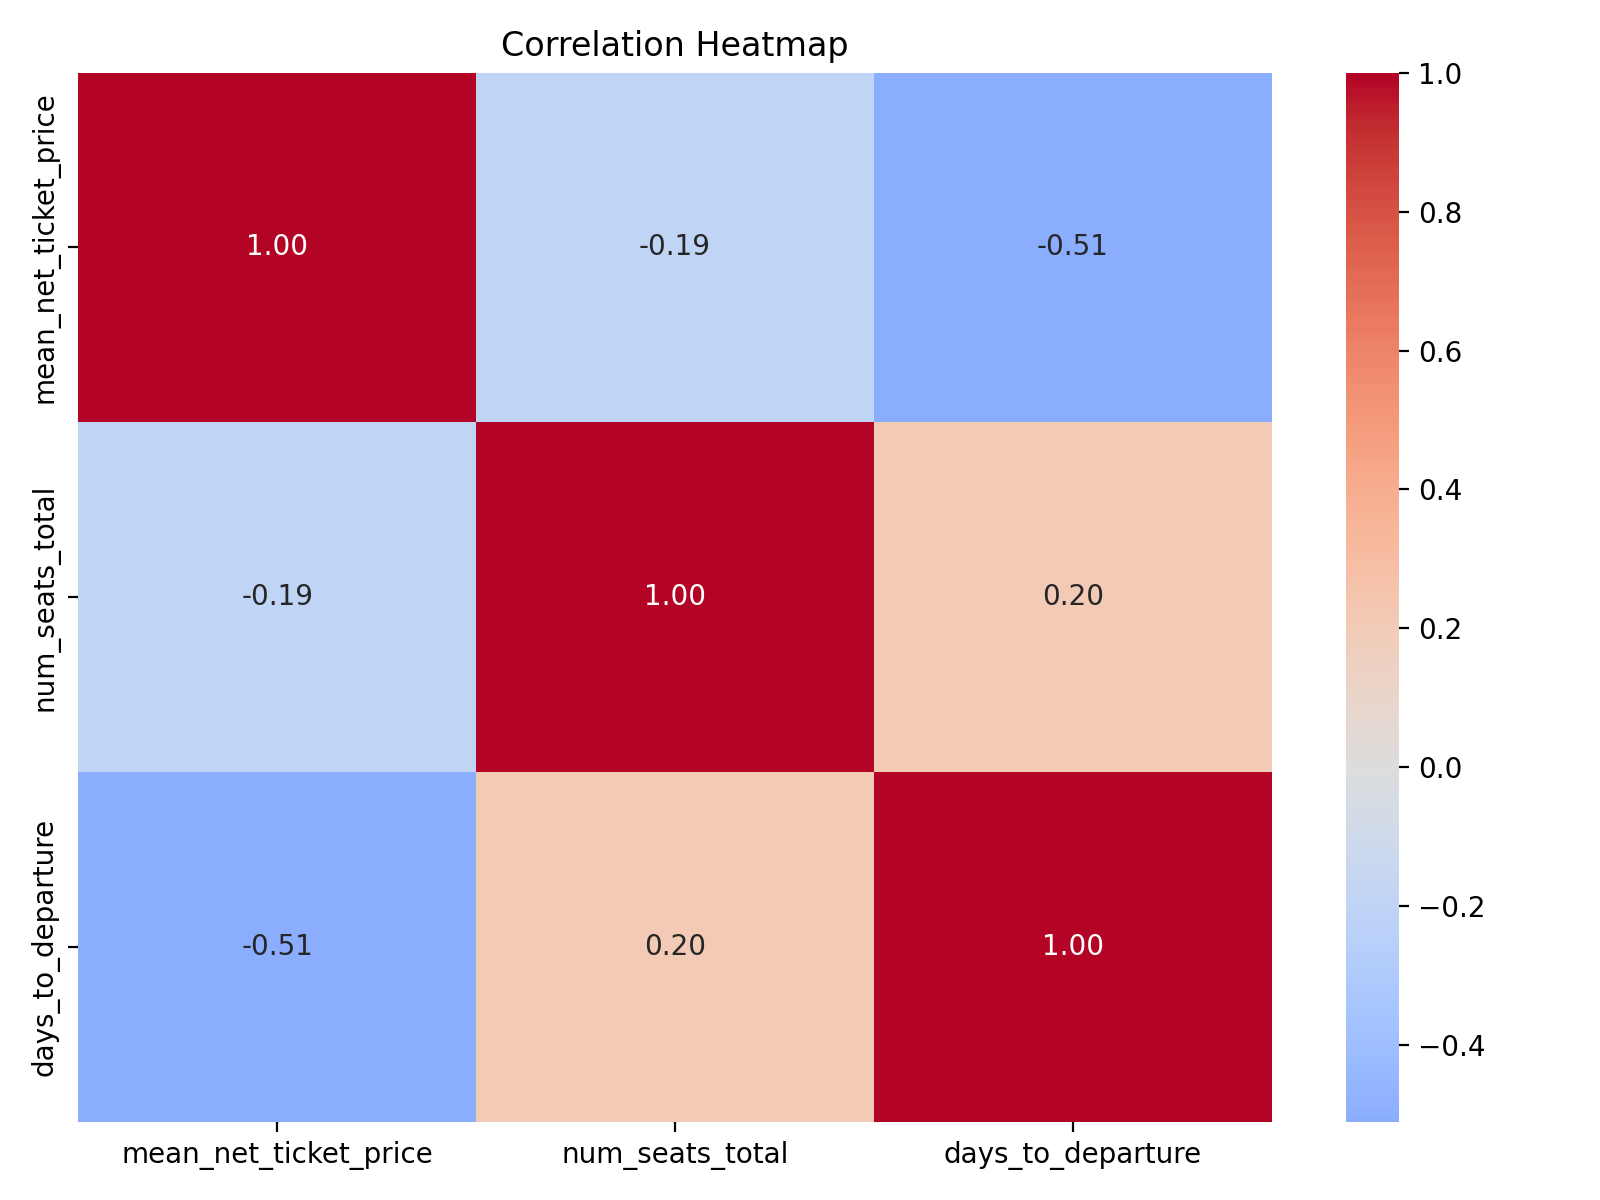
\includegraphics[width=0.8\textwidth]{booking_spec_correlation_heatmap.png}
    \caption{\small Correlation Heatmap: Price, Quantity, Days to Departure}
    \label{fig:correlation_heatmap}
\end{figure}

\textbf{Specification Testing:} We tested three functional forms for incorporating booking horizon effects:
\begin{enumerate}
    \item \textbf{Linear}: Simple linear relationship with days to departure
    \item \textbf{Categorical}: Four business-quantile categories based on 5th, 20th, and 90th percentiles of booking horizon
    \item \textbf{Log}: Logarithmic transformation to capture diminishing booking horizon effects
\end{enumerate}

\begin{figure}[H]
    \centering
    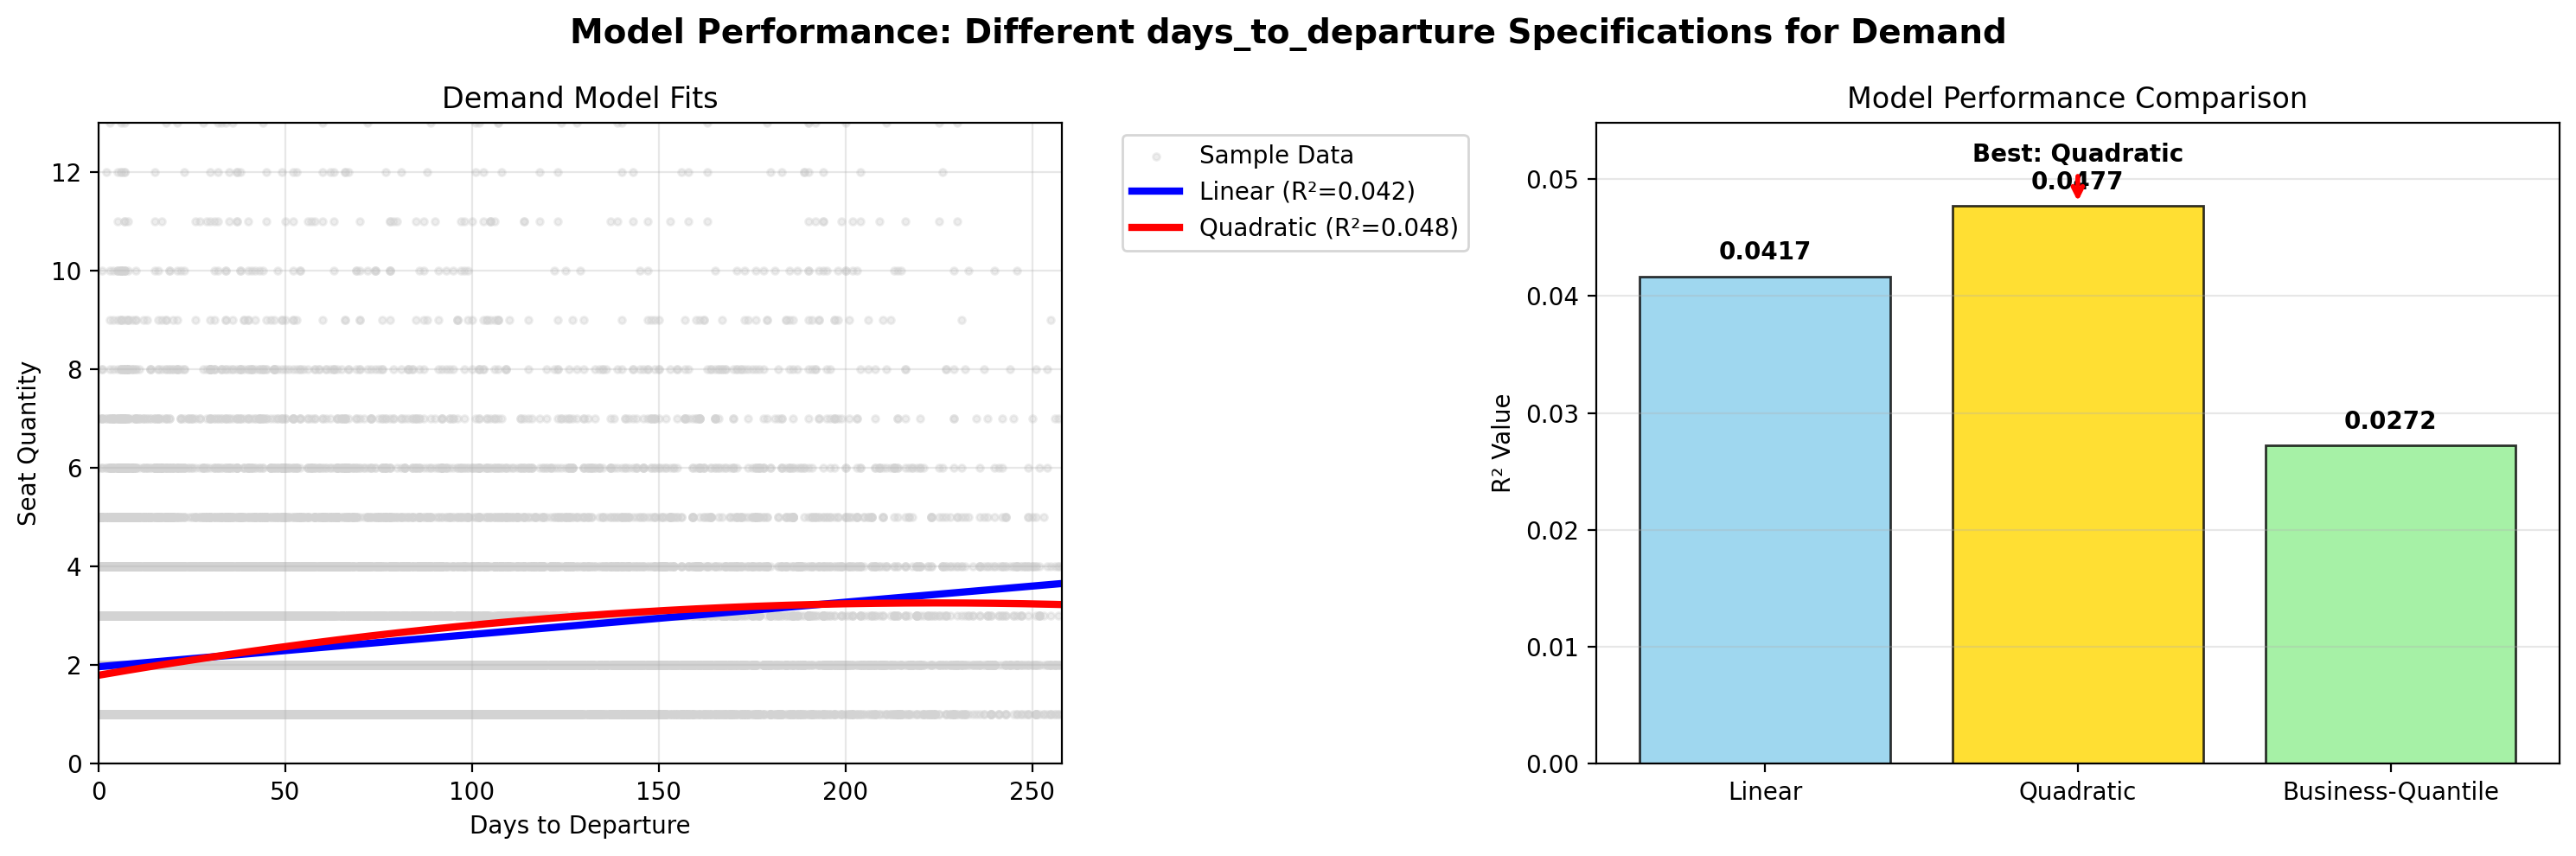
\includegraphics[width=1.0\textwidth]{booking_specifications_comparison.png}
    \caption{\small Model Performance: Different \textit{days\_to\_departure} Specifications for Demand}
    \label{fig:demand_specifications}
\end{figure}

\begin{figure}[H]
    \centering
    
\includegraphics[width=1.0\textwidth]{booking_specifications_price_comparison.png}
    \caption{\small Model Performance: Different \textit{days\_to\_departure} Specifications for Price}
    \label{fig:price_specifications}
\end{figure}

\textbf{Performance Analysis:} Our empirical testing reveals distinct patterns for demand versus price prediction. For demand estimation, performance differences between specifications are negligible (linear R² $\approx$ 0.042 vs log R² $\approx$ 0.037) - essentially indicating that booking horizon has minimal explanatory power for seat demand regardless of functional form. However, for price prediction, log specification demonstrates significantly superior performance, better capturing the non-linear relationship between booking horizon and dynamic pricing.

\textbf{Methodological Justification:} Since our 2SLS identification strategy relies on price prediction for instrumental variable strength, the superior performance of log specification in price modeling drives our functional form choice. The negligible demand performance differences confirm that our specification decision is methodologically sound rather than driven by demand-side optimization.

\textbf{Specification Consistency:} Using log specification consistently across both demand and price equations simplifies interpretation and avoids ad-hoc functional form choices based on marginal performance differences.

\newpage
\section{Choice of Seasonal Dummies over Monthly Dummies}\label{app:season_choice}

We tested seasonal versus monthly dummies as temporal variables, which serve as demand shifters in OLS and instrumental variables in 2SLS estimation.

\begin{figure}[H]
    \centering
    \includegraphics[width=0.9\textwidth]{temporal_iv_analysis.png}
    \caption{\small Temporal Instrumental Variable Analysis: Monthly vs Seasonal Patterns}
    \label{fig:temporal_iv_analysis}
\end{figure}

\textbf{Statistical Superiority:} Seasonal dummies demonstrate stronger instrument performance with F-statistic = 209.50 compared to monthly dummies (F-statistic = 152.38), both exceeding the \(F > 10\) threshold for instrument strength.

\textbf{Economic Rationale:} Seasonal patterns better capture supply-side operational cost cycles (heating, capacity, weather disruptions) while providing cleaner demand control variables. The four-season specification offers parsimony compared to eleven monthly dummies, reducing weak identification risks in 2SLS and multicollinearity in OLS.

Seasonal dummies thus provide superior statistical strength and economic interpretability for both estimation approaches.

\newpage
\section{Rationale for Log Transformation in Demand Specification}\label{app:log_transform}

We employ both linear and log-linear specifications to capture different elasticity patterns, with log transformation addressing key econometric and economic considerations.

\begin{figure}[H]
    \centering
    
\includegraphics[width=1.0\textwidth]{target_analysis.png}
    \caption{\small Target Variable Analysis: Distribution of Price and Quantity}
    \label{fig:target_analysis}
\end{figure}

\textbf{Distributional Issues:} The target variable \texttt{num\_seats\_total} exhibits substantial right-skewness in its raw form, with extreme values creating heteroskedasticity concerns in linear regression. Log transformation \texttt{log\_num\_seats\_total} = log(\texttt{num\_seats\_total}) normalizes the distribution and stabilizes variance across the range of observations.

\textbf{Economic Interpretation:} The log-linear specification enables direct interpretation of coefficients as elasticities. In the model log(\textit{quantity}) = $\beta_0 + \beta_1$ log(\textit{price}) + $\beta_2$ \textit{demand\_shifters} + $\varepsilon$, the coefficient $\beta_1$ represents the price elasticity of demand directly, simplifying economic analysis and comparison with economic theory.

\textbf{Heterogeneity Accommodation:} Log specification better accommodates proportional effects across different quantity levels, allowing elasticities to remain constant while absolute price sensitivity varies with the scale of demand. This is particularly relevant for train ticket sales with substantial variation in transaction sizes.

The dual specification approach thus provides both methodological robustness and enhanced economic interpretability for demand function estimation.

\end{document}